% !TeX root = ../main.tex
\chapter{Motivational Example}
\label{chap:motivationalexample}

Let us consider an autonomous car developer wanting to express that its system always stops when near a stop sign. The following example presents a property defined in the language that specifies the intended behavior of the developer.


%\vspace{2mm}
\texttt{after\_until robot.distance.stop\_sign < 1, robot.distance.stop\_sign > 1, eventually robot.velocity == 0}
%\vspace{2mm}

\textit{Translating into natural language, the property states in the first section that after the robot's distance to the stop-sign is below the value of 1 in the simulator, and in the second section that up until the distance is again above 1, then in the third section the robot velocity will eventually be equal to 0.}
%\vspace{2mm}

The specified property compiles to a Python file capable of running as a ROS node. The node listens only to relevant topics and performs the computations to verify the specified property.

\begin{figure}
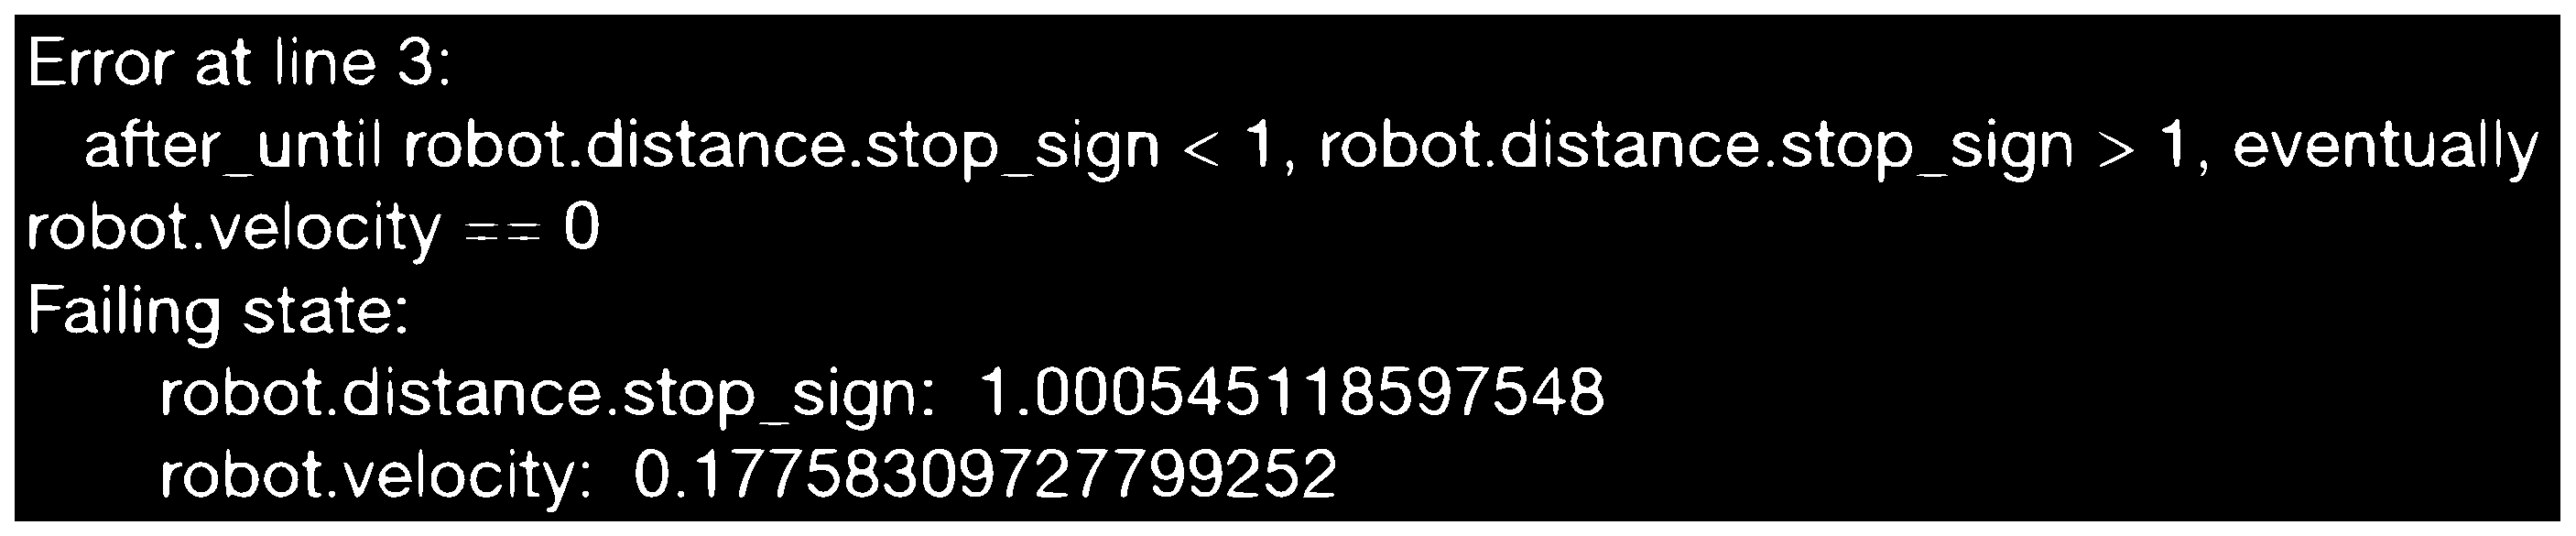
\includegraphics[width=\textwidth]{images/error.eps}
\caption{Example of the displayed error when the robot does not stop at the stop sign.} \label{fig1}
\end{figure}

The flow of the process of monitoring a robotic system is described as follows:

\begin{enumerate}[label=(\roman*)]
    \item \textbf{Property formalization:} the developer describes in the DSL the properties of the robotic system one wants to monitor in a \texttt{.txt} file extension.
    \item \textbf{Compilation:} The specified properties are compiled, and a python file is generated capable of running as a ROS node.
    \item \textbf{Monitoring:} The node can be run whenever testing the system and will listen to pertinent topics and perform the computations needed to verify the specified properties.
\end{enumerate}